\section{Correlation function results}
\label{sec:CorrelationFunctionResults}
\subsection{Combining correlation functions}
\label{sec:CFCombining}

Correlation functions have been constructed using the entirety of the LHC11h data set.  
As discussed in Section \ref{sec:CFconstruct}, events were binned in 5\% centrality bins.  
When combining data from different centrality bins, care was taken to combine the correlations by taking weighted averages of the correlation functions.  

The naive method of combining correlation functions involves adding numerators from different bins and adding denominators from different bins and then taking the ratio.  
However, this has the pitfall of potentially combining drastically different phase spaces.  
As a result, it may introduce artificial signals into the combined correlation function.  
Instead of using this method, a more correct method is to construct correlation functions for different bins separately.  
Then one takes a weighted average of the correlation functions, using the number of numerator pairs in each correlation function as the weight:

\begin{equation}
\label{eq:CombineCF}
C_{combined}(k^*) = (\displaystyle\sum\limits_{i} w_i C_i(k^*))/(\displaystyle\sum\limits_{i} w_i)
\end{equation}
where the sum is done over different correlation function bins (e.g.\ 0-5\% and 5-10\%) and $w_i$ is the number of numerator pairs in $C_i$.  
This averaging is done on a bin-by-bin basis in $k^*$.  
Note that this averaging procedure should be used in general to combine data sets with potentially different phase spaces. 
For example, this procedure is employed to combine data from runs utilizing the two different field orientations (see Section \ref{sec:DataSelection}).  
It is also employed when combining $\Lambda\Lambda$ data with $\bar{\Lambda}\bar{\Lambda}$ data.  
The statistics are too limited to analyze these correlation functions separately. Instead, we combine them together using the above method for better fitting.

For each centrality range (0-10\%, 10-30\%, and 30-50\%), the correlation functions of the two pair types were found to be consistent with each other (p-values of 0.26, 0.02, and 0.43 respectively).  
Therefore, no additional systematic error was assessed to come out of their merging.

Figures \ref{fig:CFLamLamALamALam010}, \ref{fig:CFLamLamALamALam1030STAR}, and \ref{fig:CFLamLamALamALam3050} show combined $\Lambda\Lambda + \bar{\Lambda}\bar{\Lambda}$ correlation functions for the $0-10$\%, $10-30$\%, and $30-50$\% centrality ranges respectively.  
Figures \ref{fig:CFLamALam010}, \ref{fig:CFLamALam1030}, and \ref{fig:CFLamALam3050} show $\Lambda\bar{\Lambda}$ correlation functions for the $0-10$\%, $10-30$\%, and $30-50$\% centrality ranges respectively.  
Each plot includes the combined systematic errors discussed in Section \ref{sec:SysUncertaintyCF}.
All six correlation functions are included in Figure \ref{fig:CFAllOnOnePlot}.
%, which is considered as a possible figure for publication.

\begin{figure}[hbtp]
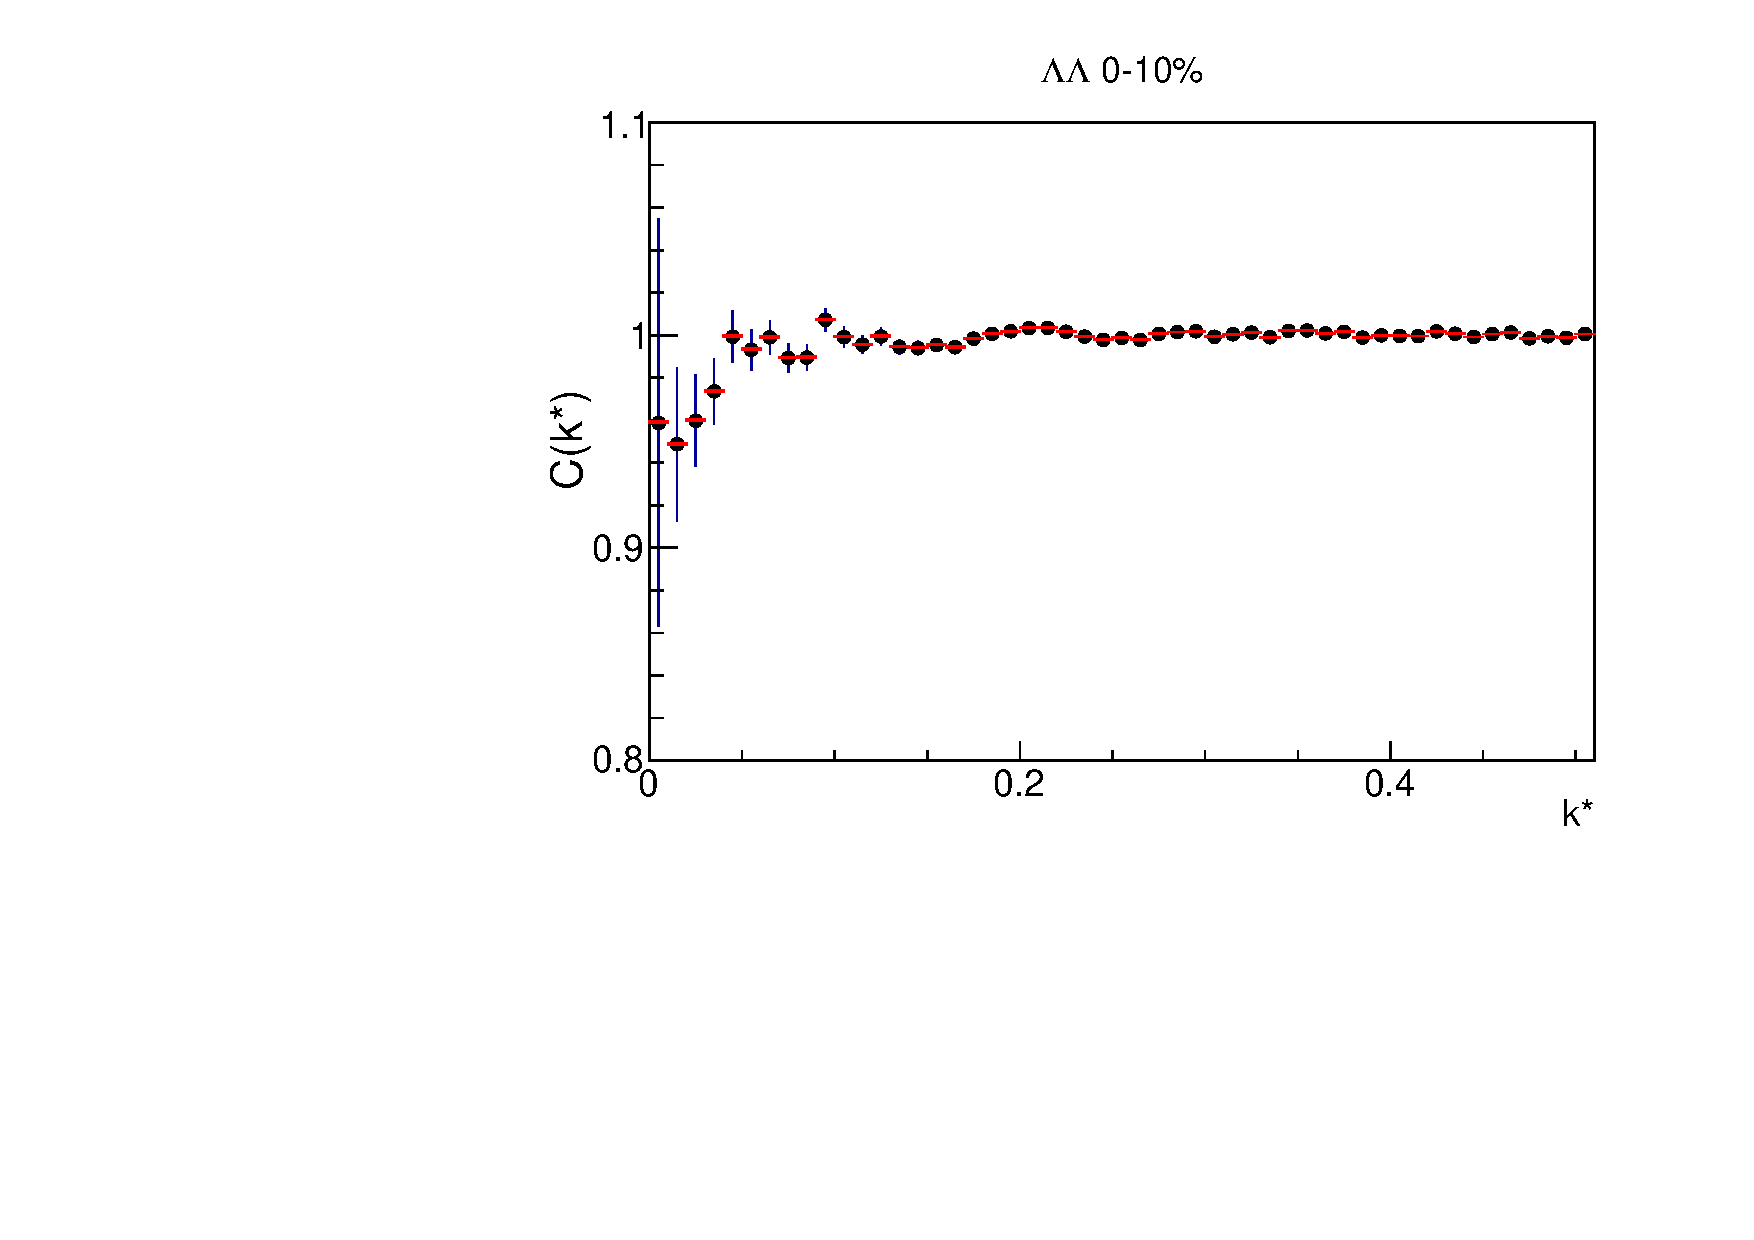
\includegraphics[width=36pc]{Figures/CFs/2016-8-30-CFLLAA010CombinedSystematicsMaximum.pdf}
\caption[$\Lambda\Lambda + \bar{\Lambda}\bar{\Lambda}$ correlation function for the 0-10\% centrality range]{$\Lambda\Lambda + \bar{\Lambda}\bar{\Lambda}$ correlation function for the 0-10\% centrality range with statistical and systematic errors.  
A dip at low $k^*$ is seen which is expected from quantum interference.}
\label{fig:CFLamLamALamALam010}
\end{figure}

\begin{figure}[hbtp]
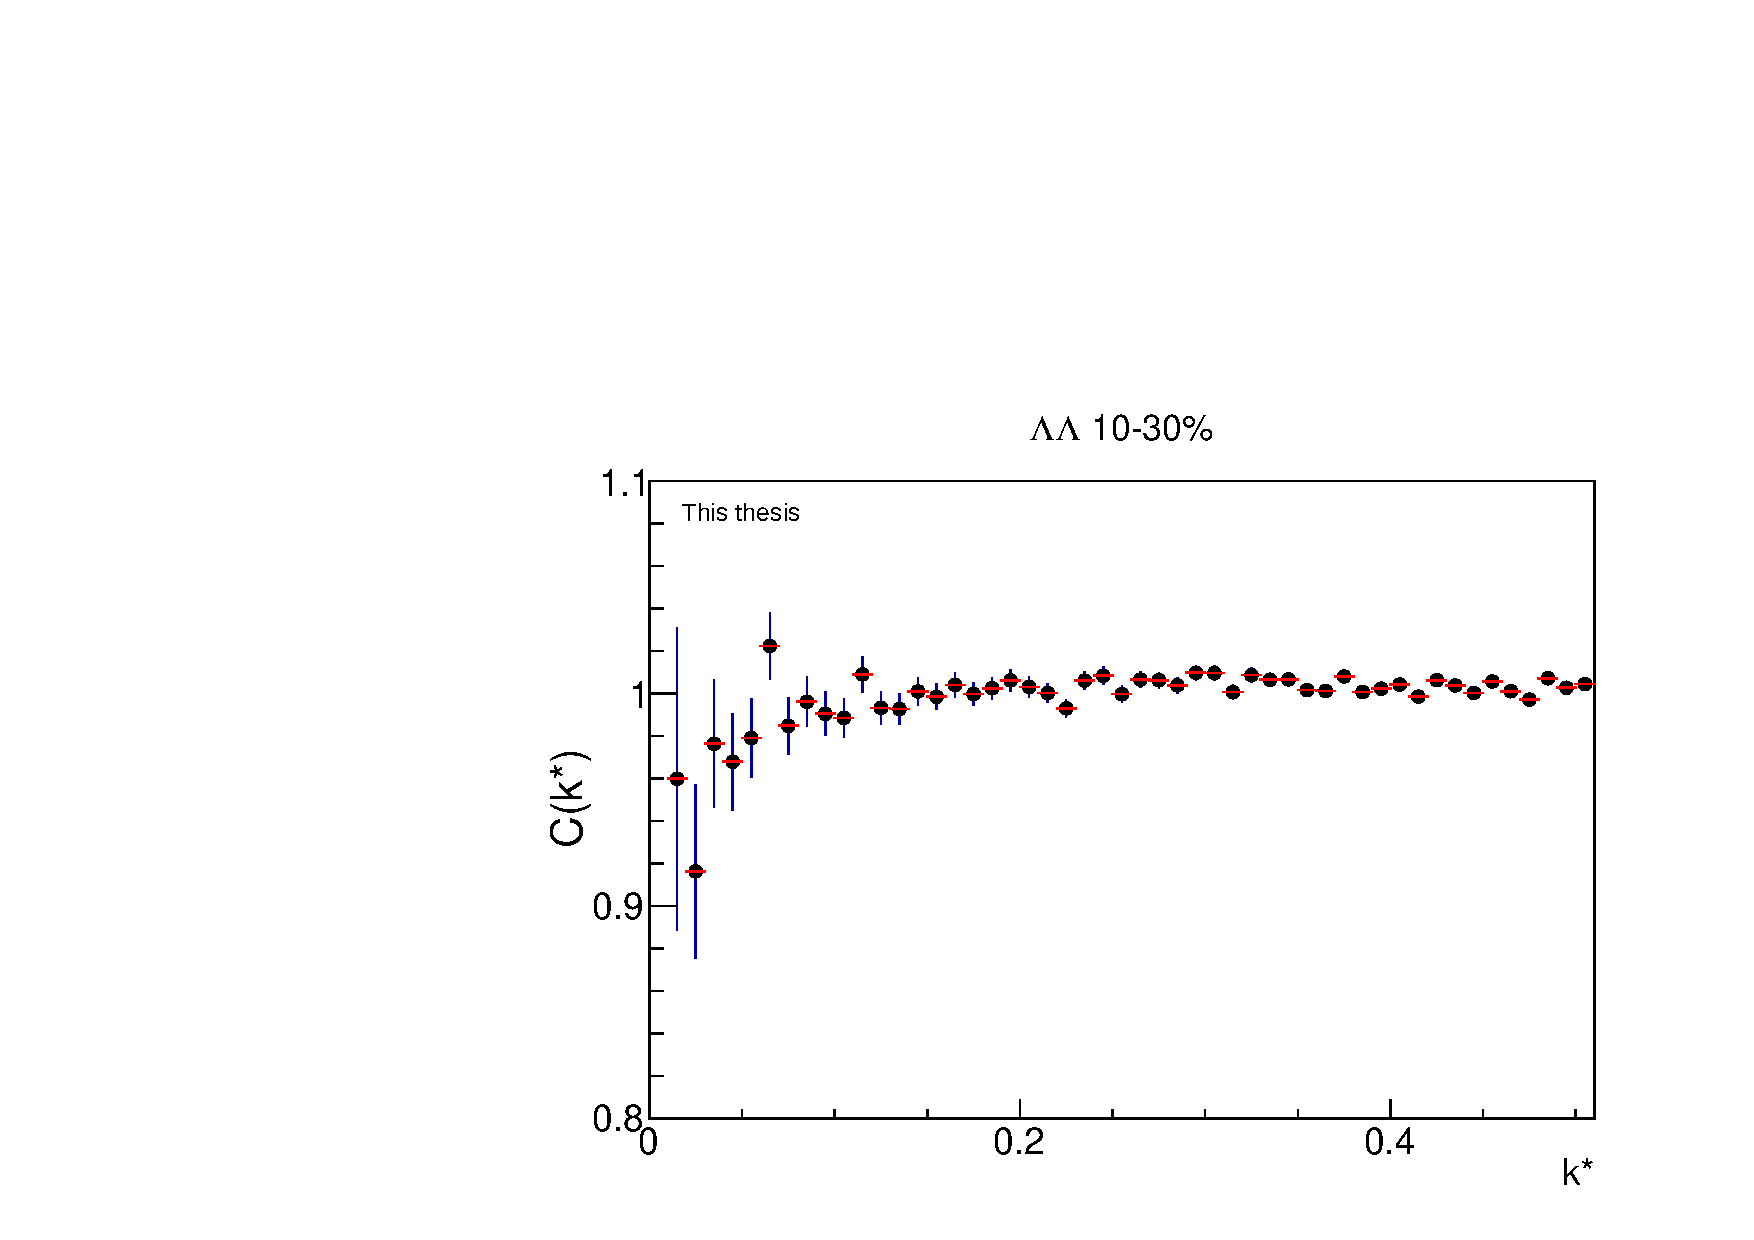
\includegraphics[width=36pc]{Figures/CFs/2016-8-30-CFLLAA1030CombinedSystematicsMaximum.pdf}
\caption[$\Lambda\Lambda + \bar{\Lambda}\bar{\Lambda}$ correlation function for the 10-30\% centrality range]{$\Lambda\Lambda + \bar{\Lambda}\bar{\Lambda}$ correlation function for the 10-30\% centrality range with statistical and systematic errors.  
A dip at low $k^*$ is seen which is expected from quantum interference.}
\label{fig:CFLamLamALamALam1030STAR}
\end{figure}

%\begin{figure}[hbtp]
%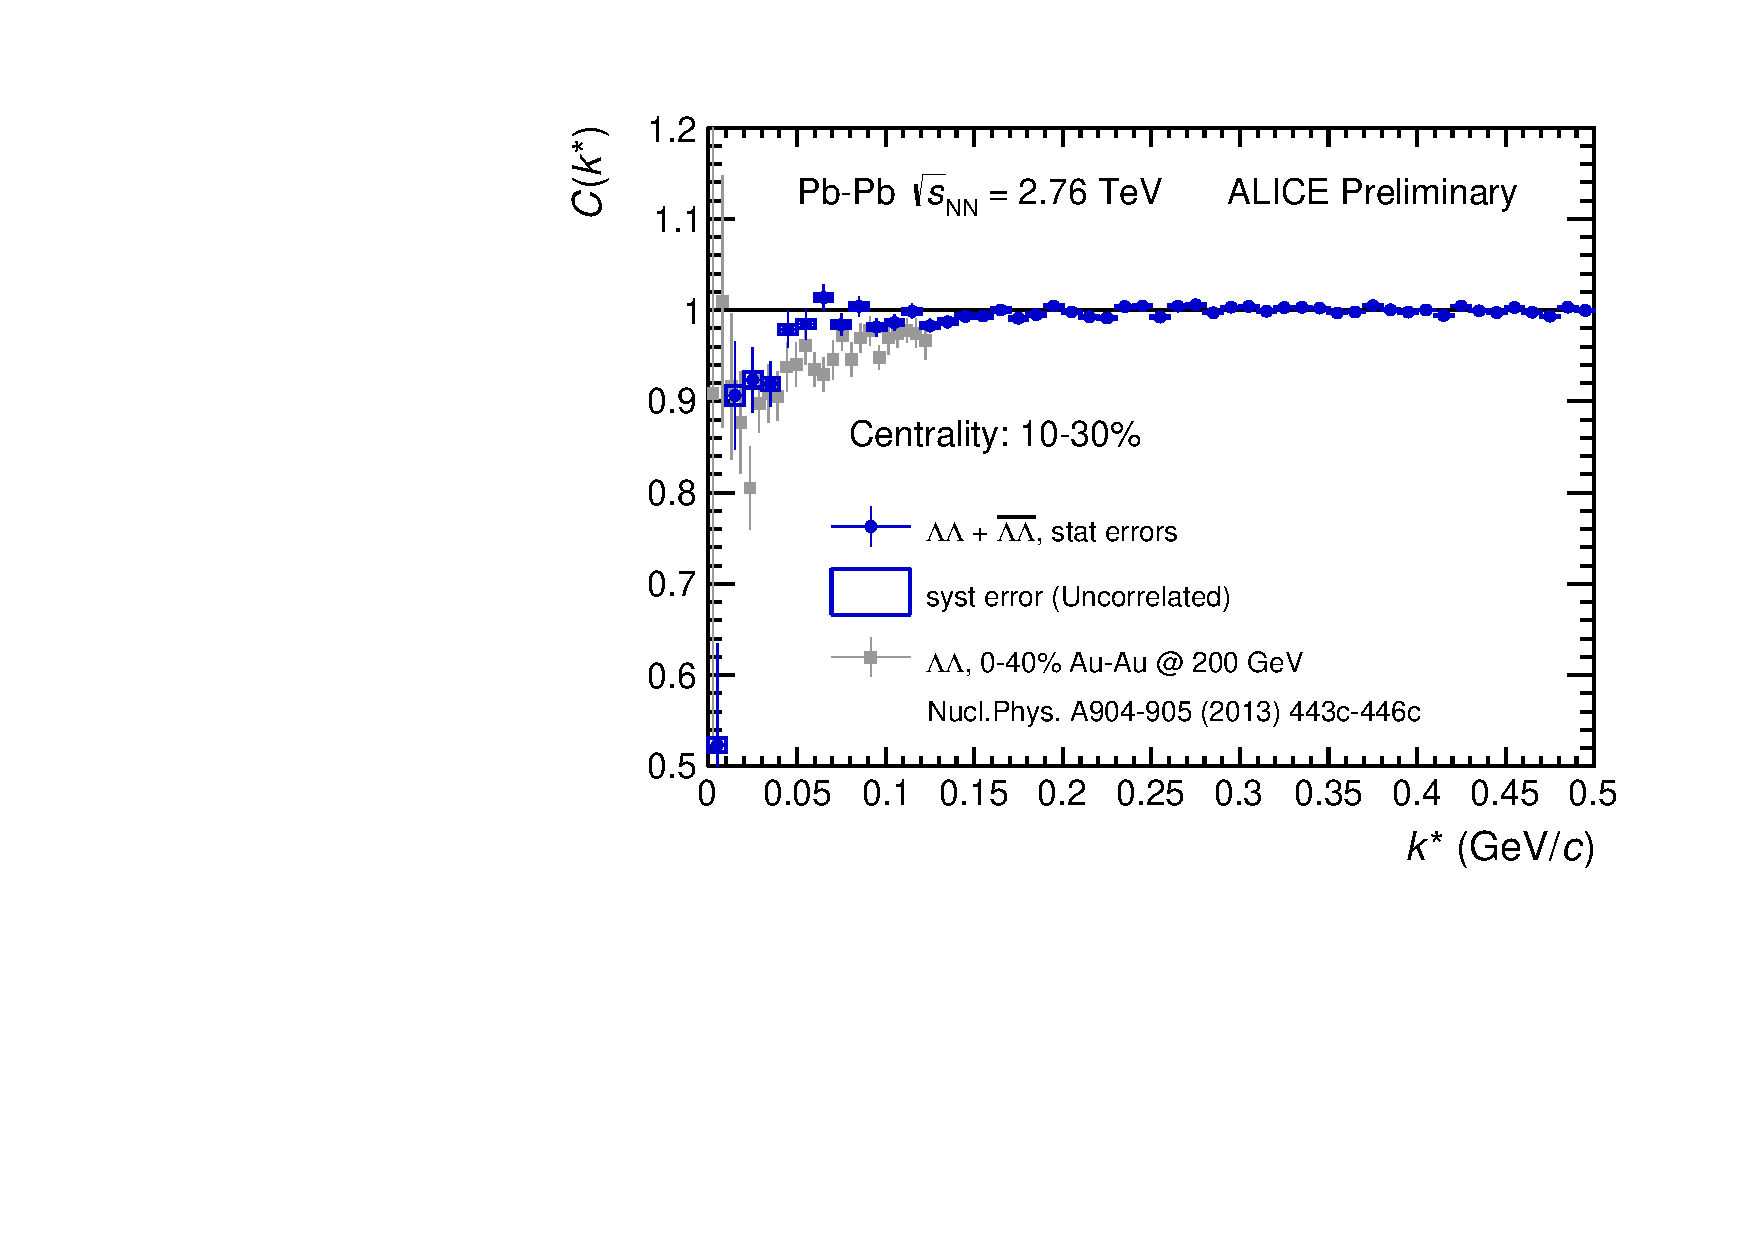
\includegraphics[width=36pc]{Figures/2014-05-11-CfLLAA-1030-CommentCorrections-WithSTAR.pdf}
%\caption[$\Lambda\Lambda + \bar{\Lambda}\bar{\Lambda}$ correlation function for the 10-30\% centrality range]{$\Lambda\Lambda + \bar{\Lambda}\bar{\Lambda}$ correlation function for the 10-30\% centrality range with statistical and systematic errors.  
%A dip at low $k^*$ is seen which is expected from quantum interference.  Preliminary STAR data for $\Lambda\Lambda$ is shown for comparison.  
%For the same plot without STAR data, see Figure \ref{fig:AppendixCFLamLamALamALam1030}.}
%\label{fig:CFLamLamALamALam1030STAR}
%\end{figure}

\begin{figure}[hbtp]
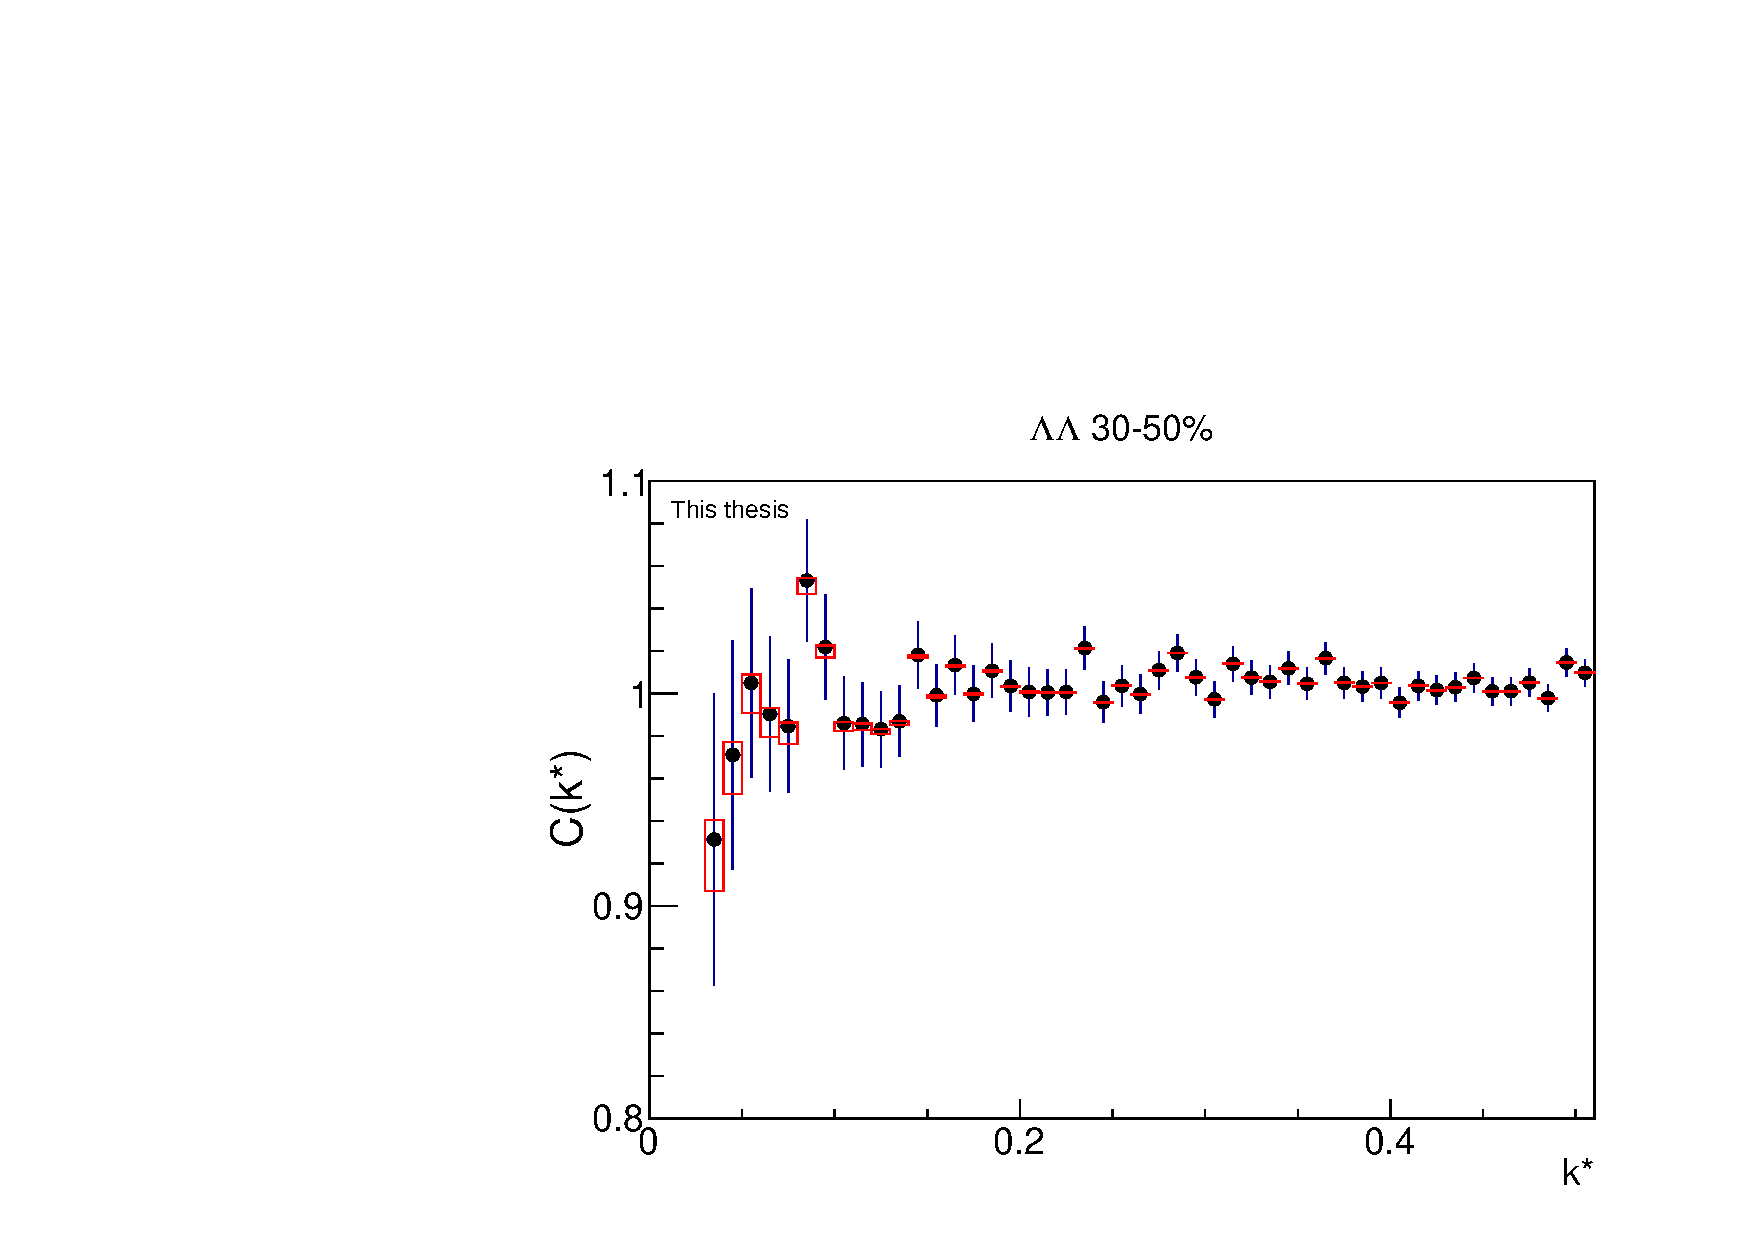
\includegraphics[width=36pc]{Figures/CFs/2016-8-30-CFLLAA3050CombinedSystematicsMaximum.pdf}
\caption[$\Lambda\Lambda + \bar{\Lambda}\bar{\Lambda}$ correlation function for the 30-50\% centrality range]{$\Lambda\Lambda + \bar{\Lambda}\bar{\Lambda}$ correlation function for the 30-50\% centrality range with statistical and systematic errors.  
Due to the poor statistics in the low $k^*$ region, it is not feasible to include this correlation function in the fit analysis.}
\label{fig:CFLamLamALamALam3050}
\end{figure}

\begin{figure}[hbtp]
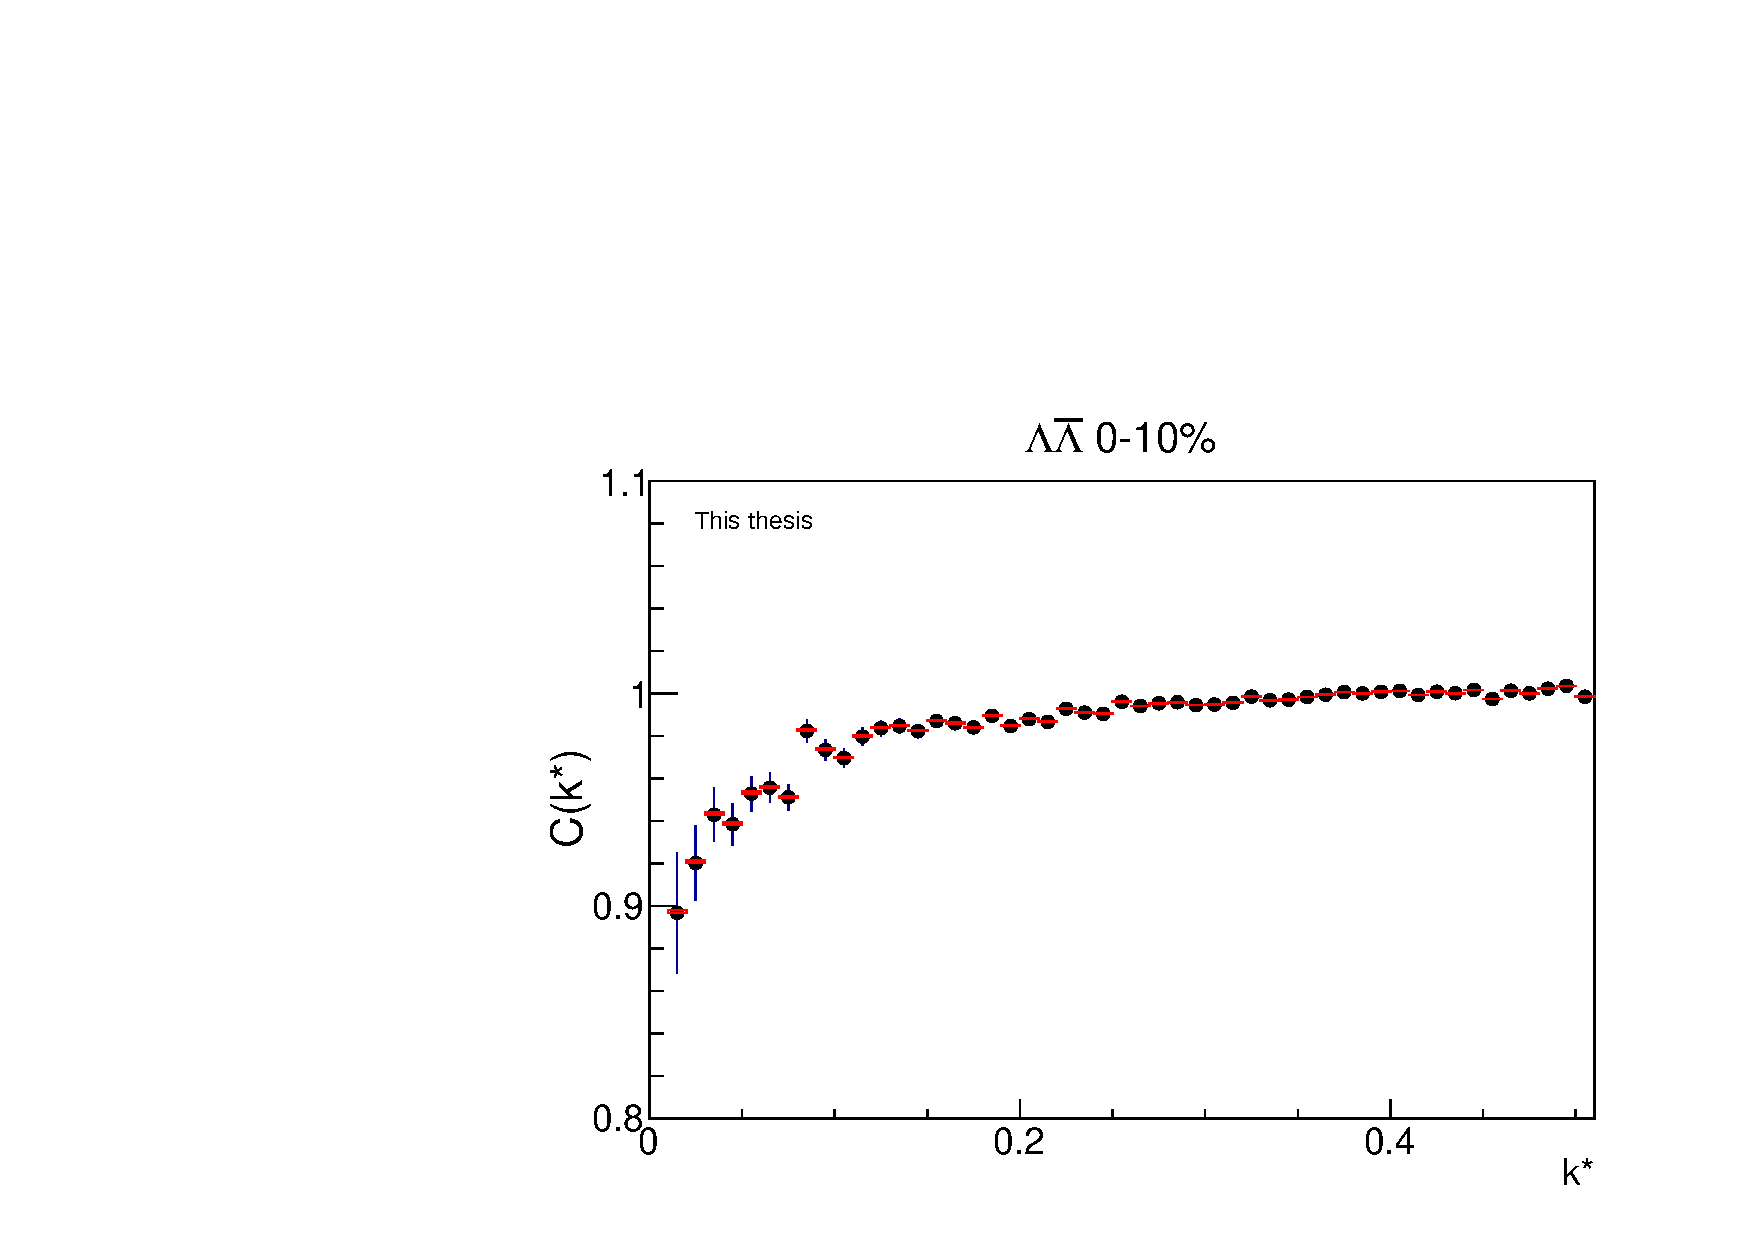
\includegraphics[width=36pc]{Figures/CFs/2016-8-30-CFLamALam010CombinedSystematicsMaximum.pdf}
\caption[$\Lambda\bar{\Lambda}$ correlation function for the 0-10\% centrality range]{$\Lambda\bar{\Lambda}$ correlation function for the 0-10\% centrality range with statistical and systematic errors.  
A wide suppression is seen which is indicative of annihilation.}
\label{fig:CFLamALam010}
\end{figure}
\begin{figure}[hbtp]
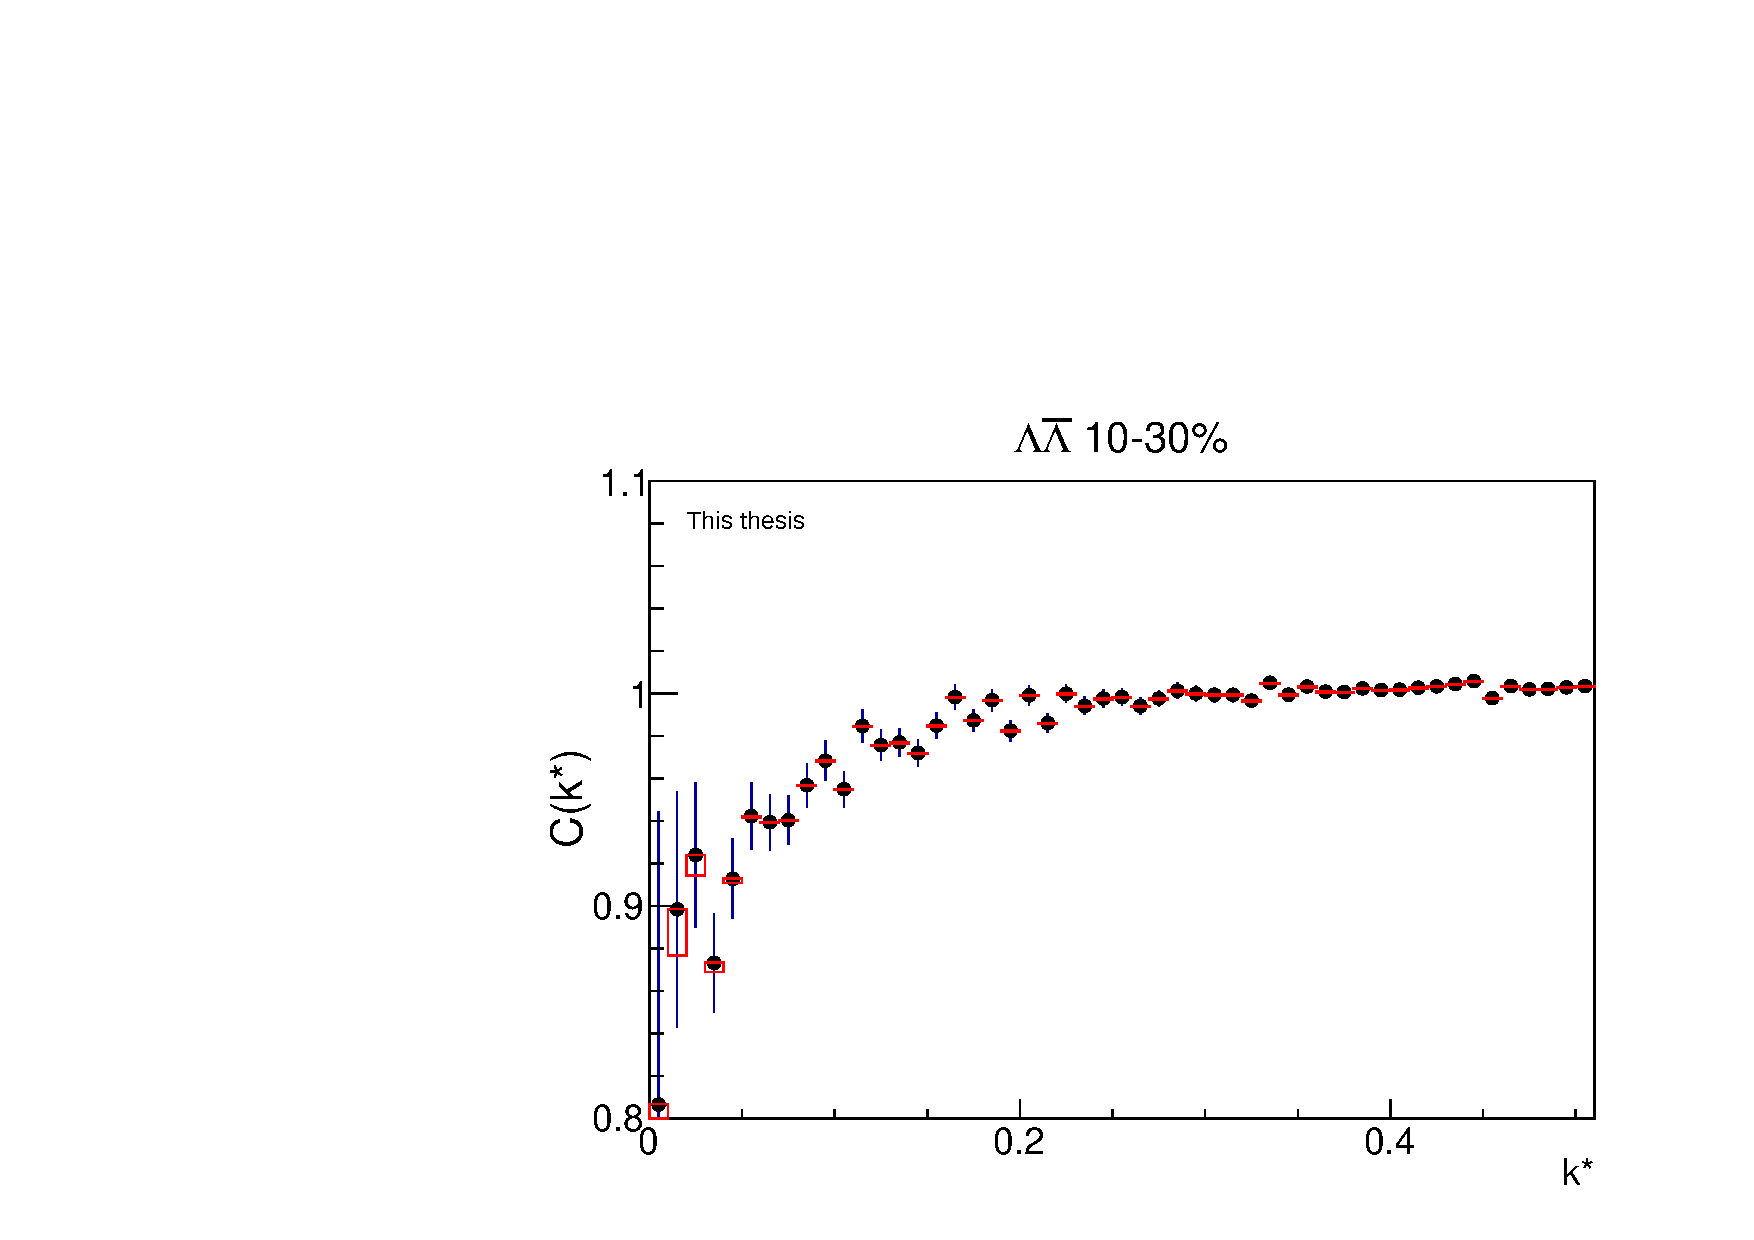
\includegraphics[width=36pc]{Figures/CFs/2016-8-30-CFLamALam1030CombinedSystematicsMaximum.pdf}
\caption[$\Lambda\bar{\Lambda}$ correlation function for the 10-30\% centrality range]{$\Lambda\bar{\Lambda}$ correlation function for the 10-30\% centrality range with statistical and systematic errors.  
A wide suppression is seen which is indicative of annihilation.}
\label{fig:CFLamALam1030}
\end{figure}
\begin{figure}[hbtp]
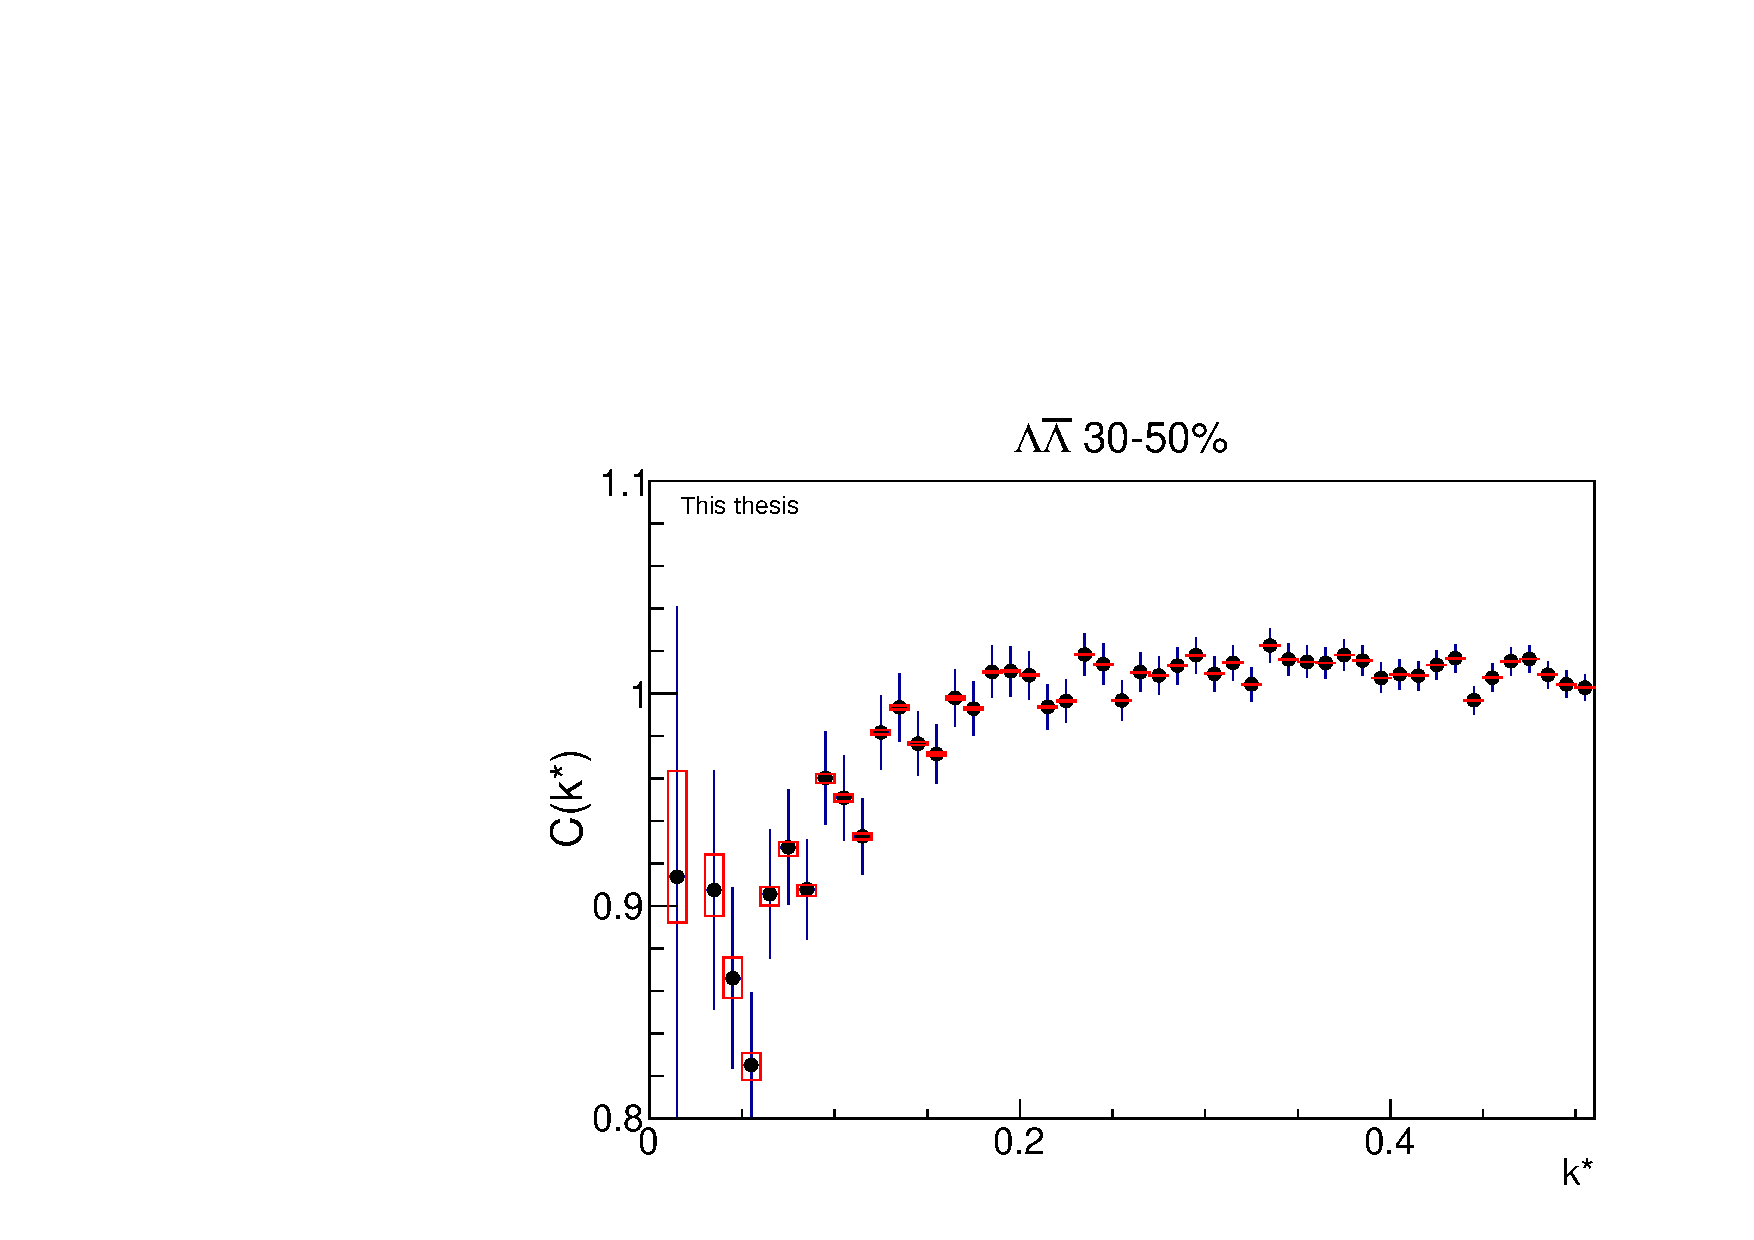
\includegraphics[width=36pc]{Figures/CFs/2016-8-30-CFLamALam3050CombinedSystematicsMaximum.pdf}
\caption[$\Lambda\bar{\Lambda}$ correlation function for the 30-50\% centrality range]{$\Lambda\bar{\Lambda}$ correlation function for the 30-50\% centrality range with statistical and systematic errors.  
A wide suppression is seen which is indicative of annihilation.}
\label{fig:CFLamALam3050}
\end{figure}

\begin{figure}[hbtp]
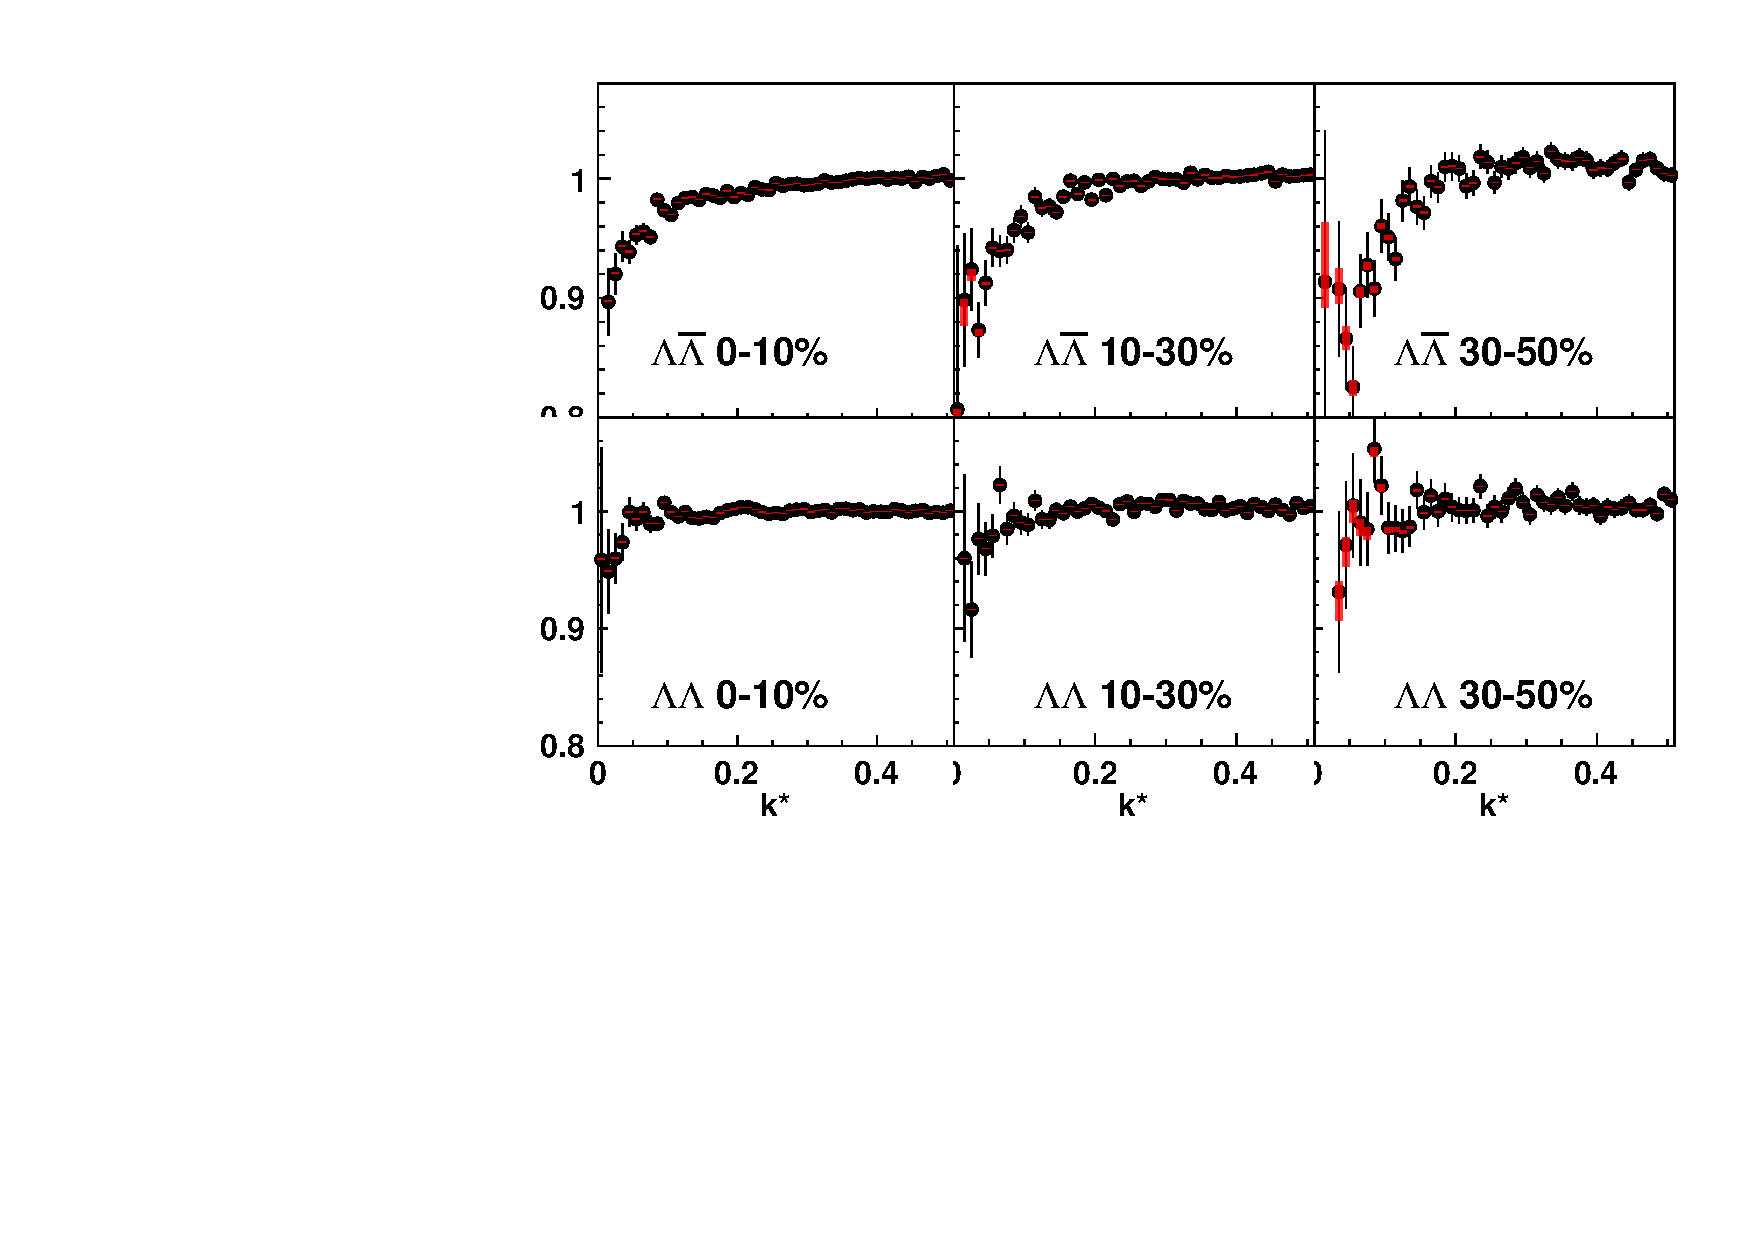
\includegraphics[width=36pc]{Figures/CFs/2016-08-30-AllCFsWithSysErrorsNoFit.pdf}
\caption[All $\Lambda\Lambda+\bar{\Lambda}\bar{\Lambda}$ and $\Lambda\bar{\Lambda}$ correlation functions]{$\Lambda\bar{\Lambda}$ (top) and $\Lambda\Lambda+\bar{\Lambda}\bar{\Lambda}$ (bottom) correlation functions for all three centrality ranges.}
\label{fig:CFAllOnOnePlot}
\end{figure}



\subsection{Interpretation of correlation function results}
\label{sec:CFInterpretation}


Generally speaking, the interesting part of a relative-momentum correlation function is the region below 100 or 200 MeV/c.  
Non-unity structures/backgrounds may be visible at large relative momentum - these structures can complicate the fitting procedure, and sometimes even direct attention to flaws in the analysis.  
They can also exist in the low-relative momentum region, though there they are generally assumed (or at least hoped) to be small.
However, the information about the source size and two-particle interactions is predominantly encoded within the low-$k^*$ region.  
For the time being, this analysis will restrict its attention to behavior in that region.
The non-femtoscopic background will be discussed more in Section \ref{sec:NonFemtoBackground}.

The $\Lambda\bar{\Lambda}$ correlation functions (Figures\ \ref{fig:CFLamALam010}, \ref{fig:CFLamALam1030}, and \ref{fig:CFLamALam3050}) exhibit a clear, centrality dependent suppression in the low-$k^*$ region, even with the significant statistical error bars for the 10-30\% and 30-50\% systems.  
A signal is also visible in the $\Lambda\Lambda + \bar{\Lambda}\bar{\Lambda}$ data, though it is smaller in magnitude and localized to a narrower $k^*$ region. 
%For reference, Preliminary STAR $\Lambda\Lambda$ results from 200 GeV Au--Au, 0-40\% centrality are also plotted \cite{Shah:2012ps}.

Several factors may contribute to the small size of this signal.  
First of all, the physics of the identical particle systems (see Sec.\ \ref{sec:AnalyticModel}) is expected to be confined to just the few lowest bins.  
There may be competing physics effects -- a suppression from quantum interference and an enhancement from the strong final state interactions -- that wash each other out.  
Furthermore, two-track effects like splitting and merging show up in this region, though they are assumed to be well-corrected for by the aforementioned pair-wise cuts.  
The presence of residual correlations may also muddle or dilute the signal region.  
This will be discussed further in Section \ref{sec:Residual}.  
%Finally, it must be noted that these are the $k^*$ bins with the least statistics.  
%There are also a couple of fitting tricks that can be employed to mitigate the statistical limitations in these plots.  
%They will be discussed in Section \ref{sec:MinuitFit}.

%********Outdated****** some of this may be salvageable

%Figure \ref{fig:CFMixCentralities} shows $\Lambda\bar{\Lambda}$ correlation functions versus $q_{\rm inv}$ for three different centralities ranges.  The correlations are normalized to unity in the $ 0.3 < q_{\rm_{inv}} < 0.5$ GeV/c range.  Each correlation shows clear suppression in the low-$q_{\rm_{inv}}$ region, which is considered an effect of the baryon-antibaryon annihilation channel.  The strength of the correlation effect increases with more peripheral events, an indication that the emitting source size is shrinking for those events.

%Figure \ref{fig:CF} shows correlation functions constructed in the 0-10\% centrality range for $\Lambda\Lambda$ and $\bar{\Lambda}\bar{\Lambda}$ pairs.  Both correlation functions exhibit an enhancement in the low-$q_{\rm inv}$ range of 0.04 - 0.2 GeV/c.  This may be due to attractive final state interactions.  The effects of FSI and quantum statistics are expected to be seen in roughly the same $q_{\rm inv}$ range, and it is unclear at this time to what extent their effects should be competing. The enhancement of the $\bar{\Lambda}\bar{\Lambda}$ correlation function does fall off in the lowest bins, though the statistical uncertainties are such that no significant statement about the effects of quantum statistics can be made at this time.



